\documentclass[12pt,oneside,abbrevs,dtc,mscres,neuro,notimes,logo,a4paper]{styles/infthesis}

% Packages
\usepackage{graphicx}
\usepackage{abbrevs}
\usepackage{acronym}
\usepackage{minted}
\usepackage{multirow}
\usepackage{wrapfig}
\usepackage{cite} 
\usepackage{gensymb}
\usepackage{amsmath}
\usepackage{mathtools}
\usepackage{tikz}
\usepackage{pgfplots}
\usepackage{scalefnt}
\usepackage{subfig}
\usepackage{tabularx}
%\usepackage{subcaption}
\usepackage{array}
%\usepackage{pgffor,pgf}
\usepackage{psfrag}
\usepgflibrary{plothandlers}
\usetikzlibrary{plotmarks}
\pgfplotsset{compat=newest}
\graphicspath{{images/}}

\mathtoolsset{showonlyrefs=false}

\renewcommand\theFancyVerbLine{\normalsize\arabic{FancyVerbLine}}

% Project Details
\title{Characterising the effect of normal brain ageing on MEG recordings: a diagnostic tool?}
\author{Alexander McMurray}
\submityear{2014}
\date{\today}


%\newacro{PSP}{Post Synaptic Potential}
\newacro{mPSP}{miniature spontaneous Post Synaptic Potential}

\abstract{
A model of healthy ageing based on the relative powers of different spectral bands in resting-state magnetoencephalograpy (MEG) recordings was constructed by performing multiple regression of age on the relative powers. As expected the model fit the healthy subjects best (as determined by tenfold cross-validation) and the diseased patients worse (as measured by bootstrap estimates of the root mean squared error (RMSE)). The RMSE values were $14.86 \pm 2.68$ years for the healthy subjects, $22.72 \pm 3.03$ years for the Mild Cognitive Impairment (MCI) patients and $26.93 \pm 2.65$ for the Alzheimer's Disease (AD) patients. The expected negative correlation between the residuals of the model and the cognitive test scores of the patients was observed but it was very weak with $r^2$ values of 0.0146 and 0.0168 for the AD and MCI respectively. Various visualisation methods all showed that the classes were not separable. This was corroborated by the poor performance of the RUSBoost classifier which only achieved an $F_{1M}$ score of 0.542 when trained on the residuals from the model (the $F_{1M}$ score using the relative powers was worse at 0.458). The $F_{1M}$ score has a maximum value of 1 for a perfect classifier while 0 is the lowest possible score. Although better than random guessing and simply guessing the majority class our classifiers lack the high specificity and sensitivity required for medical diagnosis. Future work is suggested which may lead to more successful classifiers.

}


% Extra Package Commands

\begin{document}
  \begin{preliminary}
    % Title Page
    \shieldtype{1}
    \maketitle

    % Preamble
    \begin{acknowledgements}

I would like to thank my supervisor, Dr Javier Escudero, for his guidance and support throughout the project and the staff of the Cognitive and Computational Neuroscience Lab, Centro de Tecnolog\`{i}a Biom\'{e}dica (CTB), Madrid for their kind hospitality and helpful advice. 


\end{acknowledgements}

    \standarddeclaration
    \dedication{

  % TODO: Dedication
  

}

    \tableofcontents
    \listoffigures
  \end{preliminary}

  % Chapters
  \chapter{Introduction}

 

\section{Motivation}

The twentieth and twenty-first centuries have seen a rapid increase in life expectancy but the consequent growth of the elderly population has led to an increasing prevalence of dementia.\cite{Hebert2014} Therefore the accurate diagnosis of Alzheimer's Disease (a leading cause of dementia) is an increasingly important problem.

Alzheimer's disease can be confirmed by post-mortem analysis of the brain for characteristic lesions but diagnosis of living patients depends upon neuroimaging and neuropsychological methods. Unfortunately incorrect diagnosis is common ranging from 10\% to 30\% and it is more difficult to detect earlier in the disease as the symptoms are less severe but this is also when experimental treatments are perhaps more likely to be successful. It has been noted that the lack of understanding of the normal brain ageing process remains a major challenge to accurate diagnosis but that Magnetoencephalography (MEG) remains a promising area of investigation for clinical diagnosis.\cite{Fernandez2013}

The development of reliable and objective diagnostic techniques would be invaluable to improve the selection of suitable candidates for clinical trials and thus improve the chance of discovering successful early stage treatments. An analogy can be found in cancer treatment - if clinical trials were only carried out on late Stage IV cancer patients then it would be concluded that we had very few, if any, effective treatments so the correct identification of early stage patients is vital to curing the disease. Unsurprisingly, the early detection of Alzheimer's disease has become a topic of intense focus in recent years. \cite{Nestor2004}



\section{Hypothesis and Objectives}

\begin{center}\textit{``It is a capital mistake to theorise before one has data. Insensibly one begins to twist facts to suit theories, instead of theories to suit facts.''}\\ Arthur Conan Doyle, The Adventures of Sherlock Holmes (1892)
\end{center}

The hypothesis was that Alzheimer's disease effects the normal course of brain aging, and thus a model which predicted the age of a subject from the MEG recordings which was based on healthy subject would fail when applied to Alzheimer's and MCI patients. Due to the damage that Alzheimer's causes to synapses it would seem logical to believe that the healthy model would over-estimate the true age of the patient due to the accelerated damage to the brain caused by Alzheimer's Disease. It is also assumed that the magnitude of error the healthy model had for a given patient would be proportional to the severity of their disease which can be measured by their scores on the Mini Mental State Examination (MMSE), a standard cognitive test used with Alzheimer's and Mild Congnitive Impairment (MCI) patients. The difference between Alzheimer's Disease and MCI will be discussed in the background section.

The model to be used is a multiple linear regression model with the age as the dependent variable and the relative powers of the different spectral bands averaged over different brain regions as the explanatory variables. The failure of the model can thus be quantified using the Root Mean Squared Error (RMSE) value, which can be estimated via bootstrap samples for the diseased patients and via cross-validation when obtaining the model from the healthy subjects. The classifier to be used will be a boosted decision trees algorithm that is robust to class imbalance (RUSBOOST). This will be explained in the section describing the methodology.

To summarise, the main objectives of the project were:

\begin{itemize}
\item Create a multiple linear regression model relating the relative powers of the spectral bands in the MEG recordings to the age of the subject, using healthy subjects
\item See if the failure of this model in diseased patients correlates with the severity of their condition, as measured by the RMSE value and MMSE score respectively
\item Attempt to distinguish between healthy and diseased subjects using a classifier
\end{itemize}

\section{Results Achieved}

Initially the results seemed optimistic as the RMSE values for the healthy, MCI and Alzheimer's patients showed that the model was less accurate when applied to diseased patients as hypothesised and that the magnitude of failure was worse for the more severely affected Alzheimer's group than for those with MCI, which was also as expected. However, the RMSE value of the model on healthy patients was still relatively high with the estimates having a mean of 14.86 years and a standard deviation of 2.68 years (note that this is the standard deviation of the sampling distribution and thus is equivalent to the standard error of the RMSE statistic).

However, subsequent projections of the data were worrying as the classes did not appear to be separable, neither by age within a class nor between classes as a whole. This implied that perhaps the relative powers would not allow us to distinguish between the healthy subjects and diseased patients, and thus the model based on them would also lack such discriminative ability. 

This was corroborated by the classifier results which were no better than a 'dumb' classifier which simply predicts all subjects to be healthy irrespective of the data. However, given that the data processing pipeline from raw MEG signal to feature vector is very long and involves many variables such as how to perform the artefact detection, filtering, whether to include noisier signals etc. this study does not prove that the relative powers are unable to distinguish between the disease states.

It is possible that careful tweaking of the pipeline would result in success. However, as a preliminary study it demonstrates that such a task is likely to be difficult.



\newpage

\section{Outline}

The document will be structured as follows:\\
\begin{itemize}

\item \textbf{Background} - Discussion of the literature related to the topic and past work. Includes a brief introduction to Magnetoencephalography and Alzheimer's disease covering the relevant aspects of those fields.\\

\item \textbf{Methodology and Results} - Describes the work undertaken and the results obtained. Explains the processes of data cleaning, artefact rejection, feature extraction, data visualisation and attempted classification.\\

\item \textbf{Evaluation} - Interpreting and evaluating the results.\\

\item \textbf{Conclusion} - Final statements about the work and suggestions for future work.\\

\end{itemize}





  \chapter{Background}
\section{Alzheimer's Disease}
Alzheimer's Disease (AD) is the most common cause of dementia, its incidence increases with age and it afflicts 6\% of the population aged over 65. \cite{Burns2009} It is characterised by cognitive dysfunction (loss of memory, language difficulties etc.), psychiatric symptoms (depression, hallucinations and delusions) known as non-cognitive symptoms. Severe cases may be unable to perform basic living tasks such as eating and dressing unaided. AD is a terminal disease, with death usually resulting from an associated condition such as complications of pressure ulcers or pneumonia that can manifest following the muscle atrophy that is typical in late-stage Alzheimer's patients.\cite{Burns2009}

Patients may become confused and aggressive. Interestingly these disruptive episodes have been shown to follow a temporal pattern, being more frequent in the late afternoon and early evening - a phenomenon known as `sundowning'. \cite{McCann2004} There is high comorbidity between AD and vascular disease to such an extent that the traditional distinction between AD and vascular disease as two separate diseases has been called into question.\cite{Stewart2002}

The shift from the normal cognitive decline expected with healthy ageing to preclinical dementia appears to be a gradual, continuous transition. The prodromal stage of AD is referred to as Mild Cognitive Impairment (MCI), it is characterised by memory impairments that would not be expected due to normal age-related related cognitive decline in the individual given their age and educational history (both are strong correlates for memory function). The status of MCI as a legitimate prodromal stage of AD rather than simply misdiagnosis of normal decline is supported by the fact that patients diagnosed with MCI are 15 times more likely to develop AD than those without a history of MCI.\cite{Burns2009}

Diagnosis is typically performed on the basis of cognitive and memory tests - the most common being the Mini Mental State Examination (MMSE) (see Figure \ref{fig:MMSEgraph}). Neuroimaging can aid diagnosis but no single modality has been proven as an accurate screening test. Neuroimaging used in cmbination with psychological testing outperforms either alone.\cite{Burns2009}


\begin{figure}[h!]
  \centering
    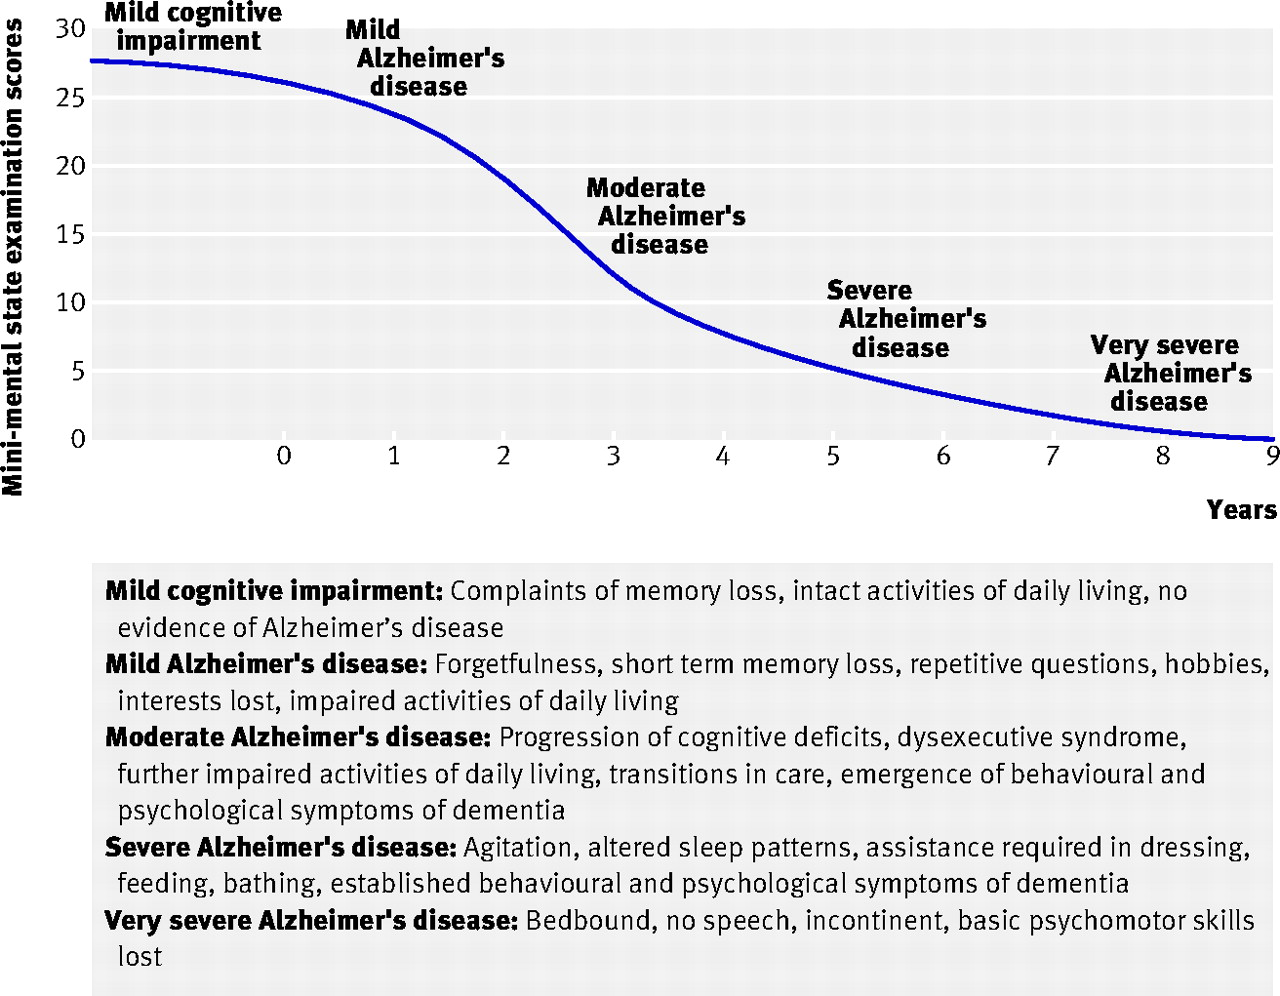
\includegraphics[width=\textwidth]{MMSEgraph.jpg}
    \caption{The progression of Alzheimer's Disease and the associated MMSE scores.\cite{Burns2009}}
    \label{fig:MMSEgraph}
\end{figure}

Although it is true that the there has been comparatively little progress in the search for an Alzheimer's cure compared to the improvement in diagnostic techniques the early diagnosis of MCI can help prevent misdiagnosis of AD and the selection of medical trial candidates. Furthermore, in the future it may allow preventative treatment to halt the progression or onset of the disease - given the modest success of late-stage intervention and the search for a cure there has been a great increase in interest concerning preventative treatment of Alzheimer's disease.\cite{Burns2009}






\section{Magnetoencephalography}

Magnetoencephalography (MEG) is a functional neuroimaging technique that measures the brain activity directly via measurement of the magnetic fields created by electrical currents at the synapses. This is a difficult task as the magnetic fields are extremely weak ($10-10^3$ fT) and thus requires the use of expensive and complicated neuromagnetometers which achieve their high sensitivity by the use of Superconducting Quantum Interference Devices (SQUIDs). Although it is worth mentioning that the first MEG recordings took place in the late 1960's before SQUIDs were available, instead using an induction coil magnetometer consisting of 2 million turns of copper wound about a ferrite core.\cite{Hari2012}

Furthermore the weakness of the magnetic fields relative to ambient magnetic noise ($10^8$ fT) requires shielding the laboratory to reduce noise. The magnetic field due to an electric current is described by Amp\`{e}re's Law and the direction can be easily determined by the right hand rule. As the magnetic field is orthogonal to the current, MEG is sensitive to the tangential component of the synaptic currents and therefore is most sensitive to pyramidal neurons near the cortical surface as pyramidal neurons have most of their currents tangential to the cortical surface and MEG is generally not sensitive to deep brain regions (although some studies have shown this may not always be the case\cite{Internationale2007}).

Despite these problems of MEG it has several advantages over other methods:

\begin{itemize}
\item It is non-invasive and has a high temporal resolution
\item Magnetic fields unlike electric fields in Electroencephalography (EEG) are not impeded by the skull, scalp etc.
\item Unlike EEG it does not require a reference signal allowing for easier source localisation\cite{Zani2002}
\item It is a direct measurement, unlike many methods such as fMRI and fNIRS which use cerebral blood flow as a proxy for neural activity

\end{itemize}

MEG recordings are often combined with anatomical MRI to enable accurate source localisation. The data processing requires the removal of artefacts which can be divided into three kinds: System related artefacts (Superconducting Quantum Interference Device (SQUID) jumps, nosiy/saturated channels etc.), external artefacts (due to power lines, mains AC etc.), physiological artefacts (due to eye movements, cardiac/muscle activity, head movement etc.). \cite{Gross2013} The visual inspection of raw data and power spectra is highly recommended although often automated/semi-automated approaches will have to be used due to the large volumes of data recorded. The way these challenges were handled in the present work will be discussed in the Methodology chapter.



\section{Previous work}


MEG has been used to investigate a wide range of brain disorders including Alzheimer's, Schizophrenia, Major Depressive Disorder and Autism. Techniques include synchrony and coherence studies (due to its high temporal resolution), Spectral ratios (the ratios of relative powers of the different frequency bands) and non-linear techniques such as complexity analysis.\cite{Williams2010}

As a result of these studies it was discovered that many brain disorders including Alzheimer's, depression, attention-deficit hyperactivity disorder and schizophrenia result in a change in the effect of ageing on brain activity as compared to healthy controls - this was described as a `rupture' in the normal evolution of the neural activity.\cite{Escudero2013}

Previous analysis on the dataset intended for use in this study found that brain oscillatory complexity (as quantified by the Lempel-Ziv Complexity algorithm) had a quadratic relationship with age.\cite{Fernandez2012} It was also discovered that spectral properties followed a similar quadratic relationship.\cite{Gomez2013}







  \chapter{Methodology}

\section{Data cleaning}

The original proposal did not allocate a great deal of time (2-3 weeks) to data cleaning (dealing with any problems the data may have and loading it into a format amenable to further processing) this turned out to be more difficult than expected and as such took significantly longer (4-5 weeks, including a visit to an MEG laboratory to learn more about the data acquisition methods and processing techniques - which proved invaluable).

Most of the data for the healthy control patients was in the same format of a text file consisting of one column per MEG channel and one column for the time vector with each sample being a separate row. However some of the subjects shared the format of the Alzheimer's and MCI patients in which each the data for each channel (and the time vector) were contained within separate folders. Furthermore, some of the subjects had their data in different units as all the data had been multiplied by a factor of $1\times10^{5}$ due to different conventions between the Spanish and English versions of Microsoft Excel which had been used to manipulate the raw data several years ago.

Eleven of the data files were corrupted. Initially it seemed that that it would be possible to still use these subjects - using interpolation to deal with the missing data and rejecting the epochs where the interpolation was used to remove any effect upon the final data. However this ended up being very time-consuming as some of the data had multiple corruptions and some was so corrupted that even attempted to partially load the data failed. Therefore as the eleven subjects represented less than 5\% of the total 233 healthy controls it was decided that it wasn't worth the time it would take to recover the data.

Almost all of the data had been downsampled at acquisition, however for reasons that remain unknown, three uncorrupted subjects and one of the corrupted ones had not been downsampled. As the desired sampling rate was known however, it was easy to downsample these subjects using the \texttt{decimate} function in MATLAB, this automatically filters the data first to satisfy the Nyquist criterion and avoid aliasing.

The \textit{Nyquist criterion} in this context refers to the requirement that the highest frequency contained in the signal is less than half of the sampling rate. If this is not the case then \textit{aliasing} will occur in which the frequency of the sampled signal does not match the frequency of the original continuous signal. This loss of information means that accurate reconstruction of the original signal is impossible. Thus prior to downsampling (reducing the sample rate), the signal is first passed through a low-pass filter with a threshold at the Nyquist frequency ($\frac{1}{2}$ of the new downsampled sampling rate) so that aliasing does not occur. \cite{Smith1999} 
It was decided to use the FieldTrip MATLAB library\cite{Oostenveld2011} designed for EEG/MEG analysis. This would make the artefact rejection easier to perform in a more rigorous and standardised manner. Unfortunately the FieldTrip library expected the data in the format output by the original MEG machine and not the format in which we had received the data. After many attempts to load the data it appeared it would not be successful and so we produced our own artefact rejection scripts in MATLAB. This proved to be unnecessary as following a discussion with the Cognitive and Computational Neuroscience group at the Centro de Tecnolog\`{i}a Biom\'{e}dica (CTB), Madrid we discovered that it was possible to `trick' Fieldtrip into loading the data provided one could provide a data header file with correct sensor information from an actual MEG machine. As the group could provide us with such a file we were then able to successfully load the data into FieldTrip and thus use it for the artefact rejection and signal processing.

The age of the subjects (and MMSE scores for the diseased patients) were stored across various different Excel spreadsheets. As these had been compiled by hand there were some typos in the filenames and differing conventions that made it impossible to fully automate the process of extracting the data into MATLAB. However it was possible to semi-automate it such that only the filenames that didn't match an entry in the spreadsheet required further inspection, reducing the number of files to check from 220 to around 40 and thus significantly reducing the time required.

\section{Artefact Rejection}

The artefact rejection process was performed in FieldTrip as mentioned previously. It is performed by computing the z-score for each point in time for each channel:

\begin{equation} z_{\textrm{ch, t}} = \frac{x_{\textrm{ch, t}} - \mu_{\textrm{ch}} }{\sigma_{\textrm{ch}}} \end{equation}

where $\mu_{\textrm{ch}}$ is the mean of the channel signal and $\sigma_{\textrm{ch}}$ is the standard deviation of the channel signal whilst $x_{\textrm{ch, t}}$ is the value of the signal in a certain channel at a certain time. 

The z-score is accumulated across all channels:

\begin{equation} zsum_t = \sum\limits^{148}_{ch=1} = \frac{z_{\textrm{ch, t}}}{\sqrt{148}} \end{equation}

where the number of channels is 148. This accumulated z-score value is compared to a threshold set by the user and if it exceeds the threshold then that epoch is rejected across all channels.


\begin{figure}[h!]
  \centering
    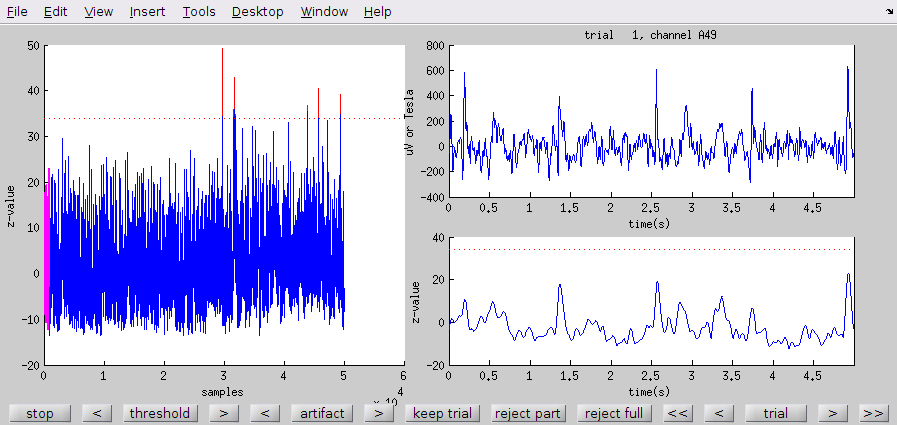
\includegraphics[width=\textwidth]{ftartefactgui.png}
    \caption{The artefact rejection GUI from FieldTrip.}
    \label{fig:ftartefactgui}
\end{figure}



Although it is possible to automate the entire process by setting a single threshold the differing noise levels between subjects meant that setting the same threshold for each subject resulted in extremely poor results. Therefore it was conducted using the manual Graphical User Interface (GUI) as shown in Figure \ref{fig:ftartefactgui}. This was quite a time-consuming process and took perhaps eight hours of solid work to process all the signals. However this approach which thresholds against the accumulated z-score was still much faster than inspecting each epoch for each channel for each patient. As there was an average of 60 5-second epochs per subject with 148 MEG channels and 278 subjects (combined total of healthy, MCI and AD) and so traditional visual inspection would have taken far too long as it would require the inspection of almost 2.5 million individual epochs.


\section{Filtering and Feature Extraction}

When the data was loaded into FieldTrip an 560th order Finite Impulse Response (FIR) filter with a Hamming window and a bandpass of 1.5 to 40Hz was applied as used by previous groups.\cite{Gomez2013}. The filter was applied to the whole signal rather than to each epoch separately to minimise edge effects (so the edge effects just occur at the first and last epochs, which can be discarded). The power spectral densities for each 5-second epoch were then obtained via Welch's method\cite{Welch1967} favoured for its noise reduction properties. See Figure \ref{fig:spectra} for an example PSD obtained from the dataset.


\begin{figure}[h!]
  \centering
    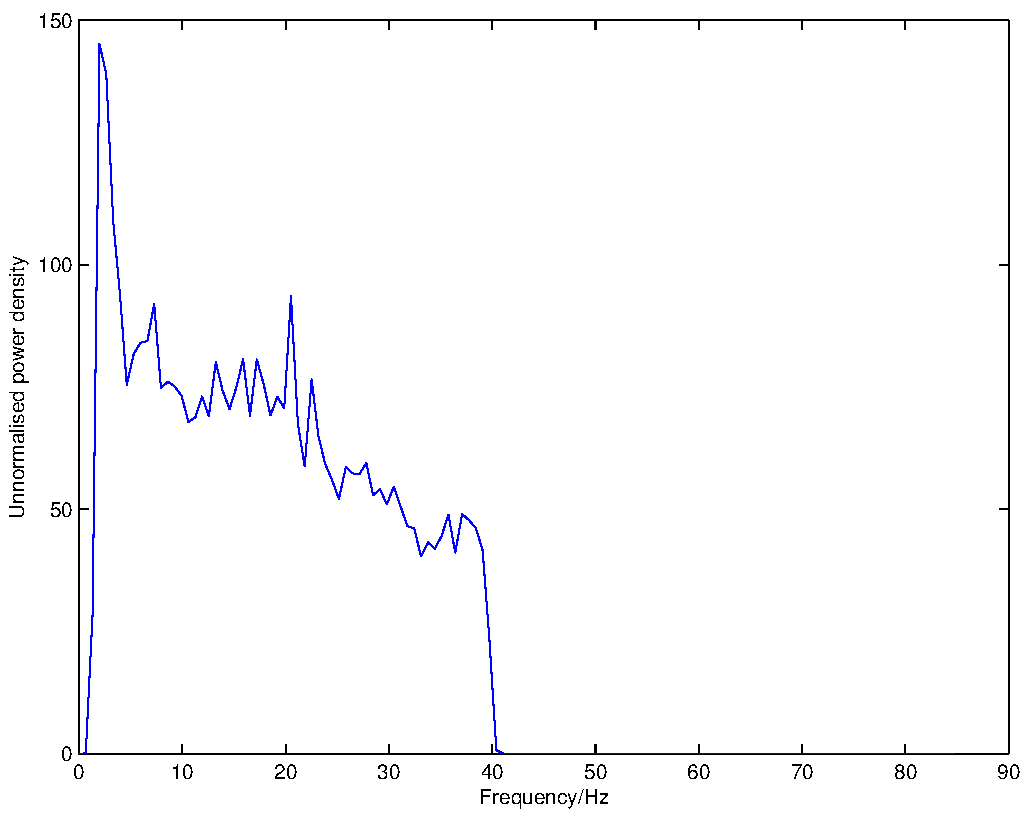
\includegraphics[width=0.8\textwidth]{postfilterexamplespectra.pdf}
    \caption{An example PSD taken from the data. Notice the sharp decline in power at 1.5 and 40 Hz due to the bandpass filter.}
    \label{fig:spectra}
\end{figure}

The relative powers were then calculated for each spectral band of interest (the conventional frequency bands associated with neural oscillations): delta (1.5-4 Hz), theta (4-8 Hz), alpha (8-13 Hz), the beta band was split into two sections - beta1 (13-19 Hz) and beta2 (19-30 Hz). The final band of interest is gamma (30-40 Hz). These are the same selection of bands used by previous groups. \cite{Gomez2013}. 

The relative powers are calculated by normalising the power spectral density (PSD) by the power contained in the total bandpass\cite{Escudero2013}:

\begin{equation} \textrm{PSD}_n(f)=\frac{\textrm{PSD}(f)}{\sum\limits^{40 \textrm{Hz}}_{f=1.5\textrm{Hz}} \textrm{PSD}(f) }   \end{equation}

and then computing the relative powers for each band from this normalised PSD:

\begin{equation} RP = \sum\limits^{f_{\textrm{high}}}_{f=f_{\textrm{low}}} PSD_n (f) \end{equation}

where $f_{\textrm{high}}$ and $f_{\textrm{low}}$ are the high and low cut-offs for the band respectively.

The relative powers were averaged over all accepted epochs and the channels were averaged into five brain regions (Central, Anterior, Left Lateral, Posterior, Right Lateral) shown in Figure \ref{fig:sensorareas}


\begin{figure}[h!]
  \centering
    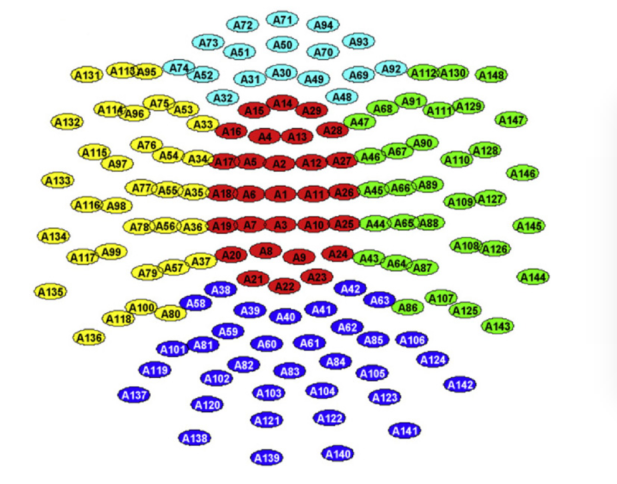
\includegraphics[width=0.8\textwidth]{sensorareas2.png}
    \caption{The division of the MEG channels into regions: Anterior (cyan), Central (red), Left Lateral (yellow), Right Lateral (green) and Posterior (blue) \cite{Escudero2013}}
    \label{fig:sensorareas}
\end{figure}

For some of the visualisations these regions were averaged over to reduce the number of features and thus the dimensionality of the data. This will be explicitly stated when the relevant visualisations are discussed. Averaging over the regions (i.e. averaging the relative powers over all channels) was also performed in previous studies \cite{Gomez2013} so it is reasonable to assume that there was not too much information lost.


\section{Model Fitting}

The features were fit with a multiple linear regression model:
\begin{equation} y = b_0 + b_1 x_1 + b_2 x_2 \cdots + b_{30} x_{30} \end{equation}
where $y$ is the dependent variable, the age of the subject, and $x_i$ are the explanatory variables (the relative powers of the different spectral bands in the different regions). The $b_i$ values are the regression coefficients, including the coefficient of the bias column of ones which was added to the feature vector in order to obtain the y-intercept of the fit.

The final model was obtained by a form of weighted model averaging. Tenfold cross-validation was used to obtain ten different models (i.e. ten sets of regression coefficients). Tenfold cross-validation involves partitioning the data into ten sets and training the model on 9 whilst using the remaining one as the test set, for all ten combinations. This prevents unrealistically optimistic error reports due to using the training data as a test set and thus provides a reasonable expectation of how well the model will generalise to unseen data. Furthermore, it is a natural means to obtain a number of models which can be used in model averaging to improve performance.

The model averaging was performed by calculating the weighted average of the regression coefficients from each model, weighted by the reciprocal of the root mean squared error (RMSE) value of each model:

\begin{equation} \vec{b}_{avg} = \frac{\sum\limits_{i=1}^{10} \vec{w}_i \vec{b}_i }{ \sum\limits_{i=1}^{10} \vec{w}_i}\end{equation}

where $\vec{w}_i = \frac{1}{\textrm{RMSE}_i}$.

Bootstrapping (i.e. sampling with replacement) \cite{Witten2011} was used to obtain an estimate of the RMSE of the averaged model on the Alzheimer's and MCI datasets. The estimates used 1000 bootstrap iterations which allows for an accurate estimation of the standard deviation of the sample distribution of the RMSE statistic (i.e. the standard error of the true distribution of the RMSE statistic). Each bootstrap set contained as many data points as in the set as a whole (so the Alzheimer's bootstraps each consisted of 39 samples and the MCI ones of 18 samples) - this is known as the \textit{0.632 bootstrap} as each set will contain 63.2\% of the unique data samples on average. It is the most common bootstrapping method. \cite{Witten2011}
\begin{table}[h!]
\begin{center}
\begin{tabular}[h!]{|c|c|c|}
\hline
Dataset & RMSE Mean & RMSE Sample standard error \\
\hline
Healthy & 14.86 & 2.68 \\
\hline
MCI & 22.72 & 3.03 \\
\hline
AD & 26.93 & 2.65\\
\hline
\end{tabular}
\caption{The RMSE values obtained on the model from each of the datasets.}
\label{tab:rmsevals}
\end{center}
\end{table}

The residuals of the model fit demonstrate the difference between the predicted age of the model and the subject's actual age. These were plotted against the subjects MMSE scores in Figure \ref{fig:cogscorecorrel} (MMSE data only available for Alzheimer's and MCI patients, not healthy subjects).

\begin{figure}[h!]
  \centering
    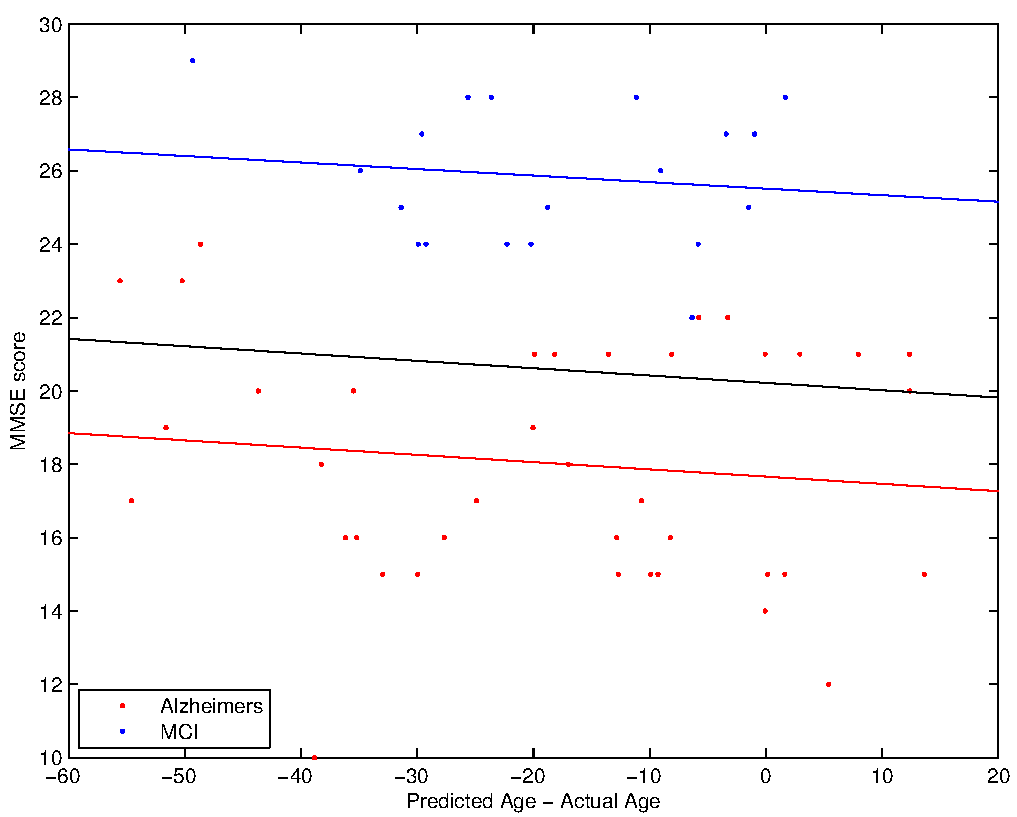
\includegraphics[width=\textwidth]{cogscorecorrel.pdf}
    \caption{The MMSE score plotted against the residuals of the model, the lines of best fit are plotted for each group. The black line is the line of best fit for the two groups combined. The correlations are very weak: the $r^2$ statistics are 0.0146 for the AD group (blue), 0.0168 for the MCI group (red) and 0.0060 for the two groups combined (black)}
    \label{fig:cogscorecorrel}
\end{figure}





\section{Data visualisation}

As the data consisted of 30 features (6 spectral bands $\times$ 5 sensor regions) it cannot easily be visualised in a two-dimensional space amenable for printing, however it is possible to project the to a lower dimensional space or to display the relationships between feature values in a different manner (in the case of the parallel co-ordinate plot).


\subsection{t-Distributed Stochastic Neighbour Embedding}

t-Distributed Stochastic Neighbour Embedding (t-SNE)\cite{Maaten2008} is a data visualisation technique that maps the original high dimensional space of the data to a lower dimensional space (usually two-dimensional by default) to allow the data to be visualised. For example, one may produce a scatter plot of the high-dimensional data once it has been projected into two-dimensions. t-SNE reduced the dimensionality of the data whilst trying to retain as much of the high-dimensional structure as possible.

 It does this by computing a similarity metric between each pair of points by centering a Gaussian on one of the points in the high-dimensional space and using the probability density as the similarity metric. A Student's t-distribution with a single degree of freedom is used in the lower dimensional space in order to provide a more convenient cost function and avoid the \textit{crowding problem} due to insufficient area in the low dimensional space to accommodate all the nearby data points whilst retaining an accurate model of small distances. The differences between the similarity metrics in the high-dimensional space and the low-dimensional map are minimised as measured by the Kullback-Leibler divergence.\cite{Maaten2008}

 Thus t-SNE has the advantages that it is able to faithfully retain both the small-scale local structure of the high-dimensional data and the long-range global structure combined with a cost function that is easier to compute than traditional SNE which used Gaussian distributions in both the high and low dimensional spaces.\cite{Maaten2008}

 For example, see the t-SNE plot for the MNIST dataset of handwritten digits shown in Figure \ref{fig:mnisttsne}. The different classes are clearly separable which shows that classification of the digits should be possible from the data given.


\begin{figure}[h!]
  \centering
    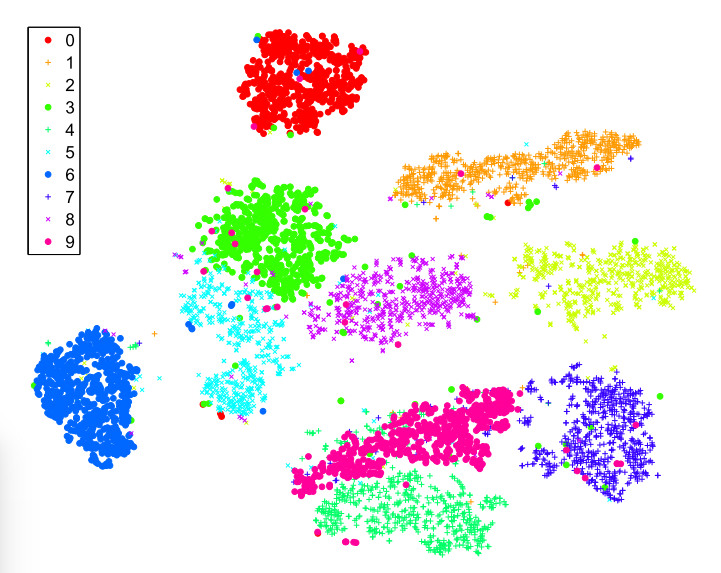
\includegraphics[width=.8\textwidth]{mnisttsne.png}
    \caption{The t-SNE visualisation of 6000 handwritten digits from the MNIST data set.\cite{Maaten2008} Note that the classes are clearly separable.}
    \label{fig:mnisttsne}
\end{figure}


t-SNE plots of each class (healthy, MCI or AD) with the samples separated by age were produced to see if within a disease group the age could be distinguished. This resulted in Figures \ref{fig:htsneplot}, \ref{fig:mcitsneplot} and \ref{fig:alztsneplot}. As can be seen in the plots the different age groups were not separable and so it does not seem as though the relative powers gave much information about age when excluding the effects of disease.


\begin{figure}[h!]
  \centering
    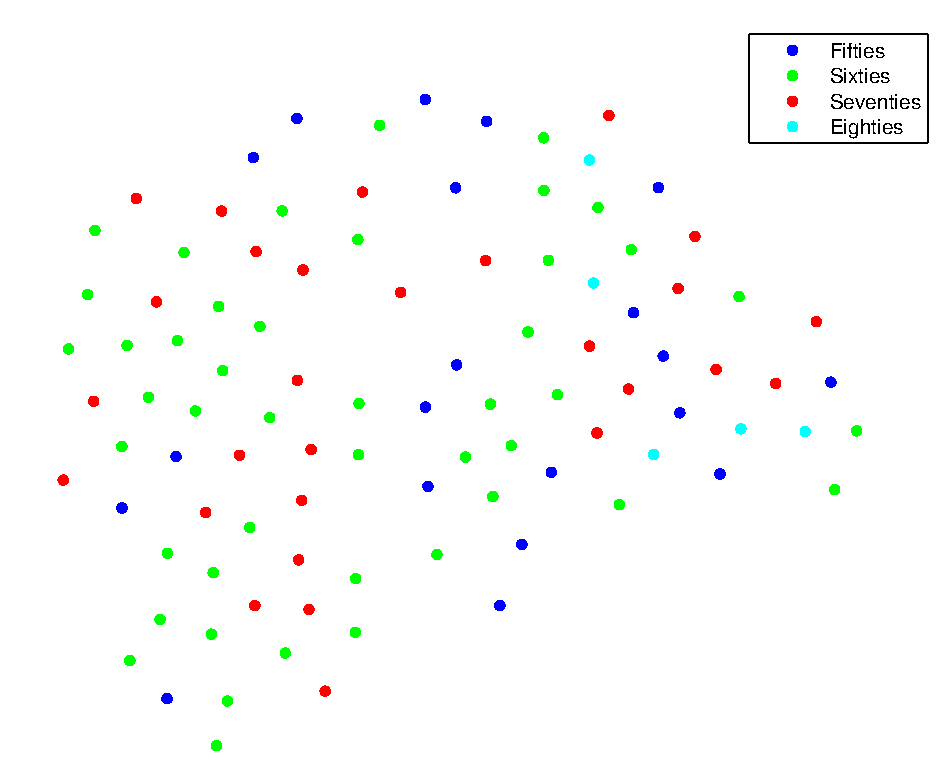
\includegraphics[width=.8\textwidth]{htsneplot.pdf}
    \caption{The t-SNE visualisation of the healthy subjects, divided into age groups. Note that the groups are not separable.}
    \label{fig:htsneplot}
\end{figure}


\begin{figure}[h!]
  \centering
    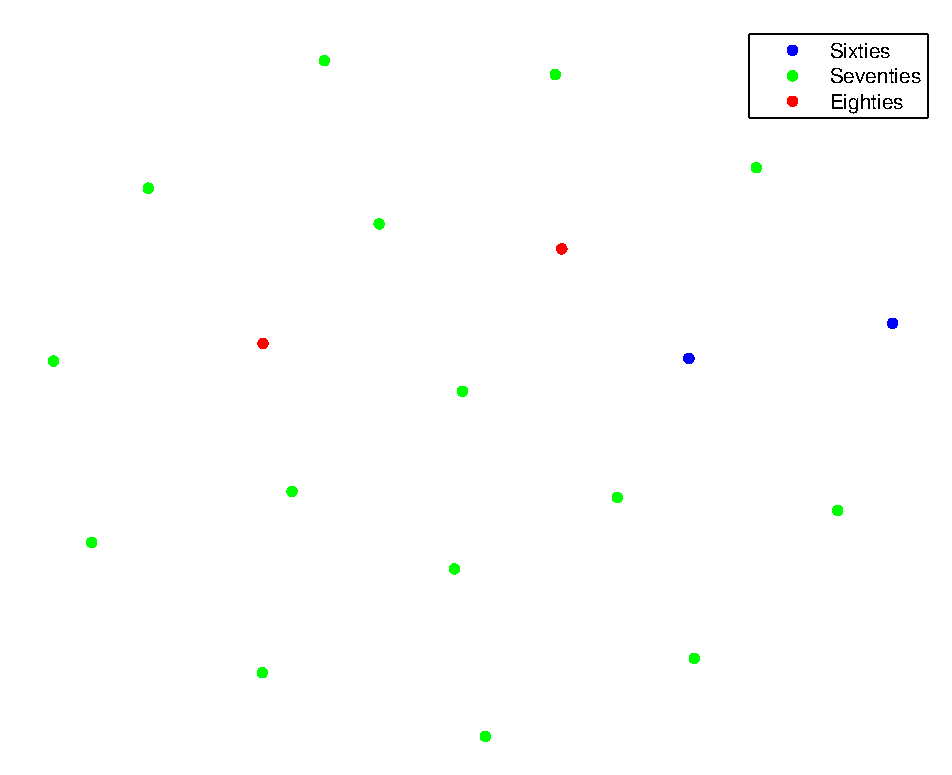
\includegraphics[width=.8\textwidth]{mcitsneplot.pdf}
    \caption{The t-SNE visualisation of the MCI patients, divided into age groups. Note that the groups are not separable.}
    \label{fig:mcitsneplot}
\end{figure}


\begin{figure}[h!]
  \centering
    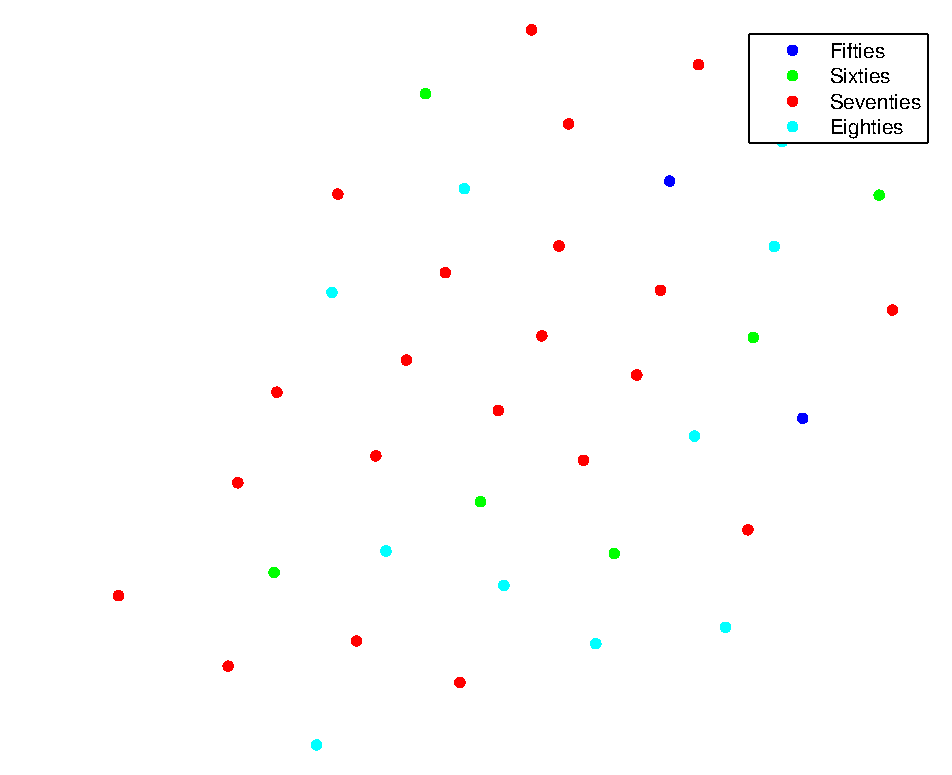
\includegraphics[width=.8\textwidth]{alztsneplot.pdf}
    \caption{The t-SNE visualisation of the AD patients, divided into age groups. Note that the groups are not separable.}
    \label{fig:alztsneplot}
\end{figure}


The total dataset was plotted to see if it was possible to distinguish between the healthy, MCI and AD subjects (see Figure \ref{fig:tottsneplot}). It did not appear to be the case, however it is possible that the effect of differing age might cause overlap between the disease groups simply due to the age difference between some members (e.g. if the young AD subjects overlapped with the old healthy ones then they would not appear as separable but it would still be possible to distinguish the classes). To take this into account we also plotted all the classes just for a single age group (subjects aged 70-79) as shown in Figure \ref{fig:seventiestsneplot}. The fact that the classes were still not separable was bad as it meant that classification would be at best difficult, if not impossible, using the given data.


\begin{figure}[h!]
  \centering
    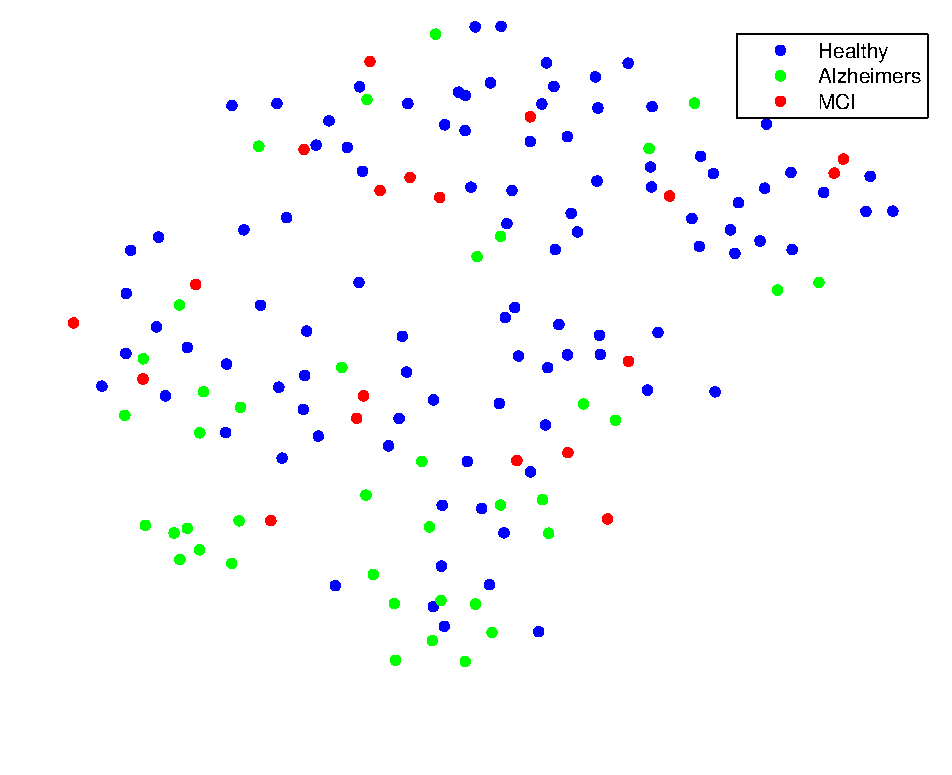
\includegraphics[width=.8\textwidth]{tottsneplot.pdf}
    \caption{The t-SNE visualisation of all the groups. Note that the groups are not separable but this could be due to the effect of age.}
    \label{fig:tottsneplot}
\end{figure}


\begin{figure}[h!]
  \centering
    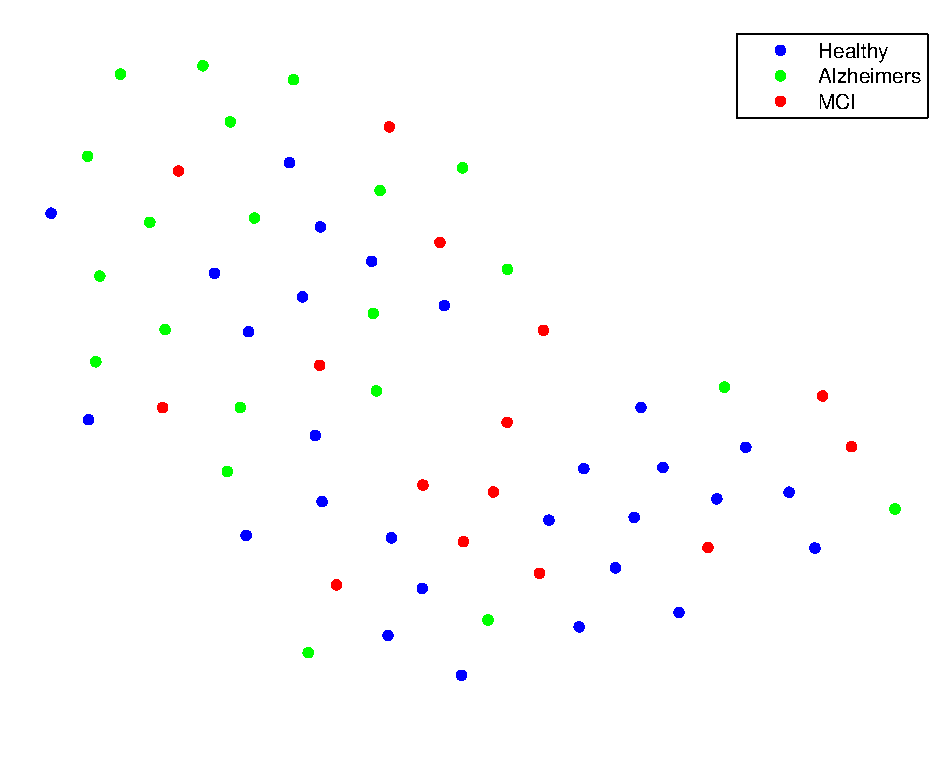
\includegraphics[width=.8\textwidth]{seventiestsneplot.pdf}
    \caption{The t-SNE visualisation of the all the groups, only subjects aged 70-79. Note that the groups are not separable. This implies classification will be difficult if not impossible.}
    \label{fig:seventiestsneplot}
\end{figure}

\clearpage


\subsection{Principal Components Analysis}

In contrast to the non-linear dimensionality reduction of t-SNE, Principal Components Analysis (PCA) is a linear projection of the data onto lower dimensional axes oriented such that the maximal amount of variation of the high dimensional data is preserved. \cite{Bushati2011} It is computed from the principal eigenvectors of the covariance matrix of the data. However PCA prioritises maintaining large-scale global structure over local structure in the data and so although the distances between distant points are well depicted, information contained within the distances between local points may be lost as the distances between proximal points are not as well depicted.

An advantage to PCA is that it still has defined axes whereas t-SNE just displays the pairwise similarity between points via the separation between them. Although the PCA axes may not always be physically meaningful (as it is just a linear combination of the original features) it can be useful to know which of the original features are responsible for most of the variance in the data and this information can be extracted from the principal components.

For the PCA plots the data used was a reduced feature set of six features: the spectral bands averaged over all brain regions. This was done such that the projections of the original axes could also be placed onto the plot so that it was possible to easily see which features contributed the most to the principal components - if this had been done with the full set of 30 features the plot would have been much too crowded. The plots are two-dimensional scatter plots using the first two principle components (i.e. the two that explain the most variance) because three-dimensional plots are difficult to clearly interpret when printed as one cannot rotate them so they may be misleading.

Plots were produced for the healthy dataset across all age groups as shown in Figure \ref{fig:pcahealthyplot} and for all classes across all age groups as shown in Figure \ref{fig:pcatotalplot}. These were not separable and as their t-SNE plots were not separable either and t-SNE is generally believed to be better at retaining the inherent high dimensional structure of the data\cite{Bushati2011} there seemed little benefit in including the other plots which just had the same result.

\begin{figure}[h!]
  \centering
    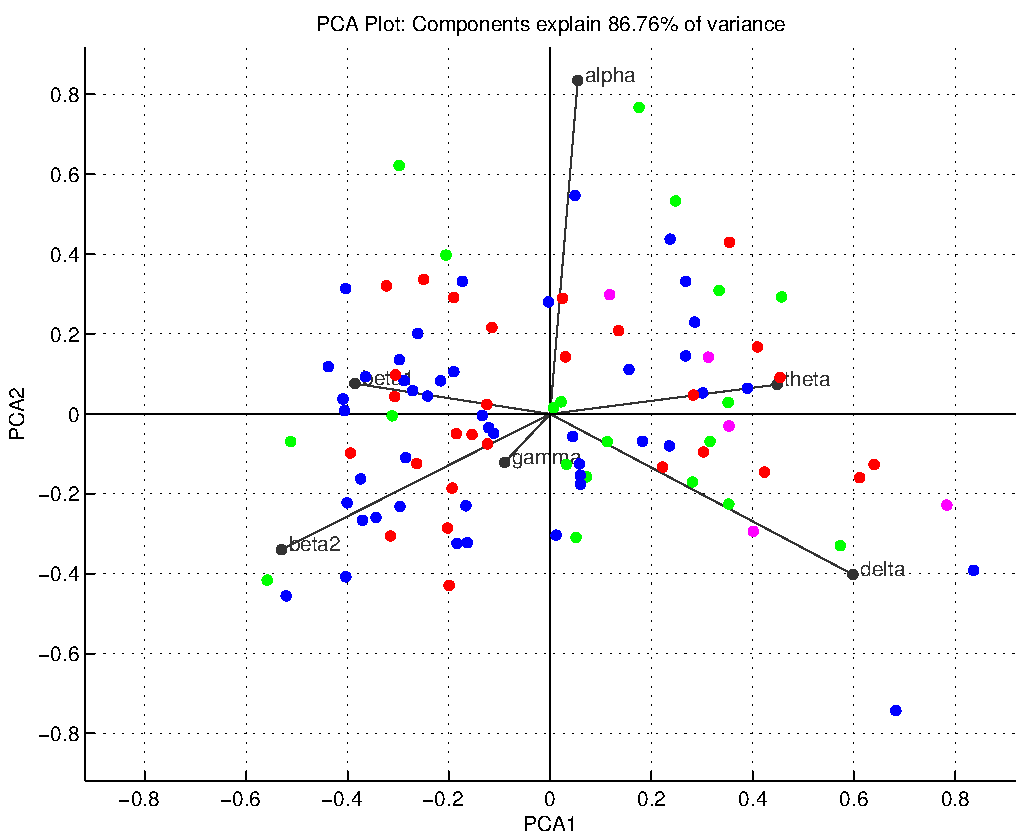
\includegraphics[width=\textwidth]{pcahealthyplot.pdf}
    \caption{The PCA projection of the healthy dataset, the two principal components explained 86.76\% of the data. The age groups following age groups were plotted: 50-59 (green), 60-69 (blue), 70-79 (red), 80-89 (magenta). Note that the groups are not separable.}
    \label{fig:pcahealthyplot}
\end{figure}

\begin{figure}[h!]
  \centering
    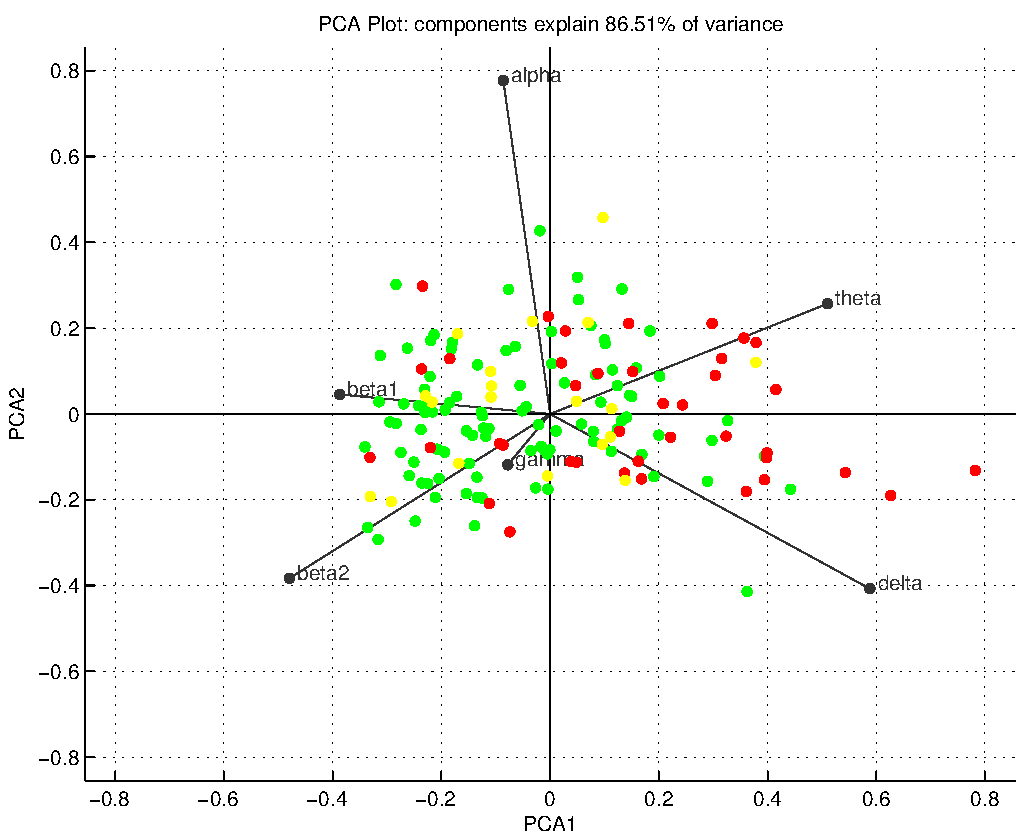
\includegraphics[width=\textwidth]{pcatotalplot.pdf}
    \caption{The PCA projection of the total dataset, the two principal components explained 86.51\% of the data. The classes are displayed as follows: Healthy (green), MCI (yellow), Alzheimer's Disease (red). Note that the groups are not separable.}
    \label{fig:pcatotalplot}
\end{figure}


\clearpage
\subsection{Parallel Coordinates plots}

A popular method to investigate the relationships between variables is the Parallel Coordinates Plot (PCP). It can also be used to examine the differences between classes and has had many applications ranging from optimising manufacturing to economic modelling \cite{Inselberg1997}.

The PCPs were produced using the reduced feature set (the same as used for the PCA plots) so that the axes could be reasonably spaced.

In the PCP each polyline represents a datapoint and it intercepts the axes at the value it has in the dimension represented by that axis. Therefore parallel lines between axes indicate a positive correlation between them, where crossing of lines in an X-shape indicates a negative correlation and random crossing indicates little or no relation.\cite{Inselberg1997}

\begin{figure}[h]
  \centering
    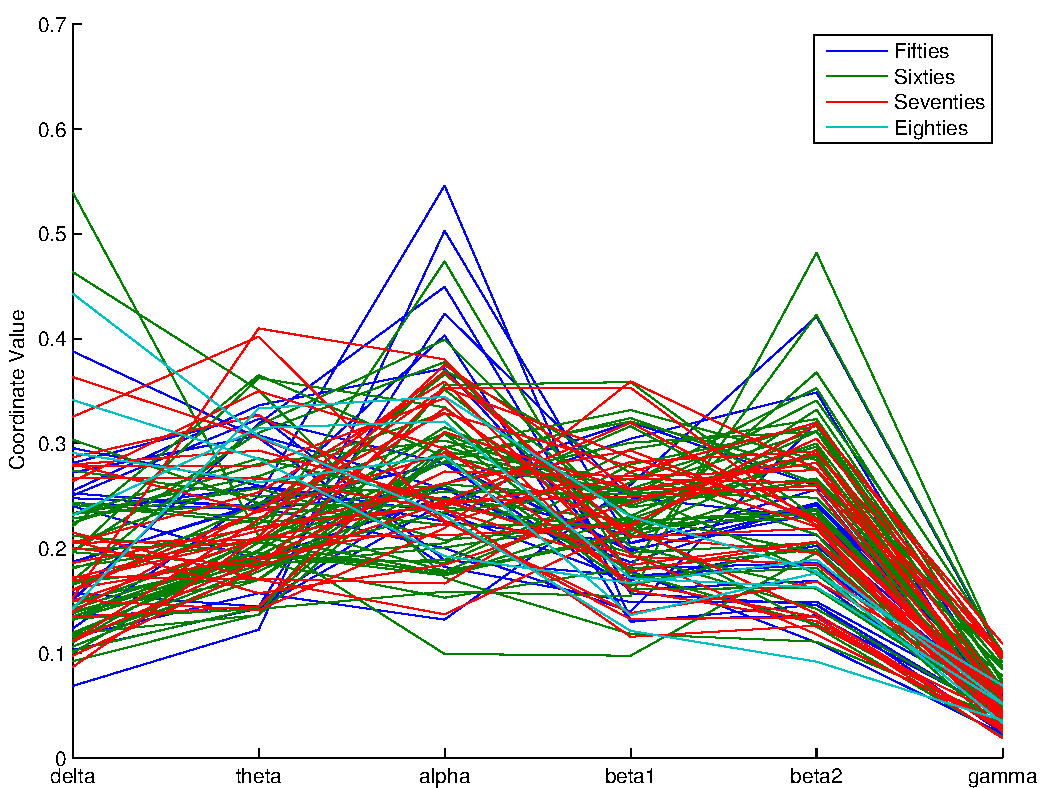
\includegraphics[width=.8\textwidth]{hparacoords.pdf}
    \caption{The Parallel Coordinate Plot of the healthy dataset divided into different age groups, there is no discernable pattern or separation between them}
    \label{fig:hparacoords}
\end{figure}


\begin{figure}[h]
  \centering
    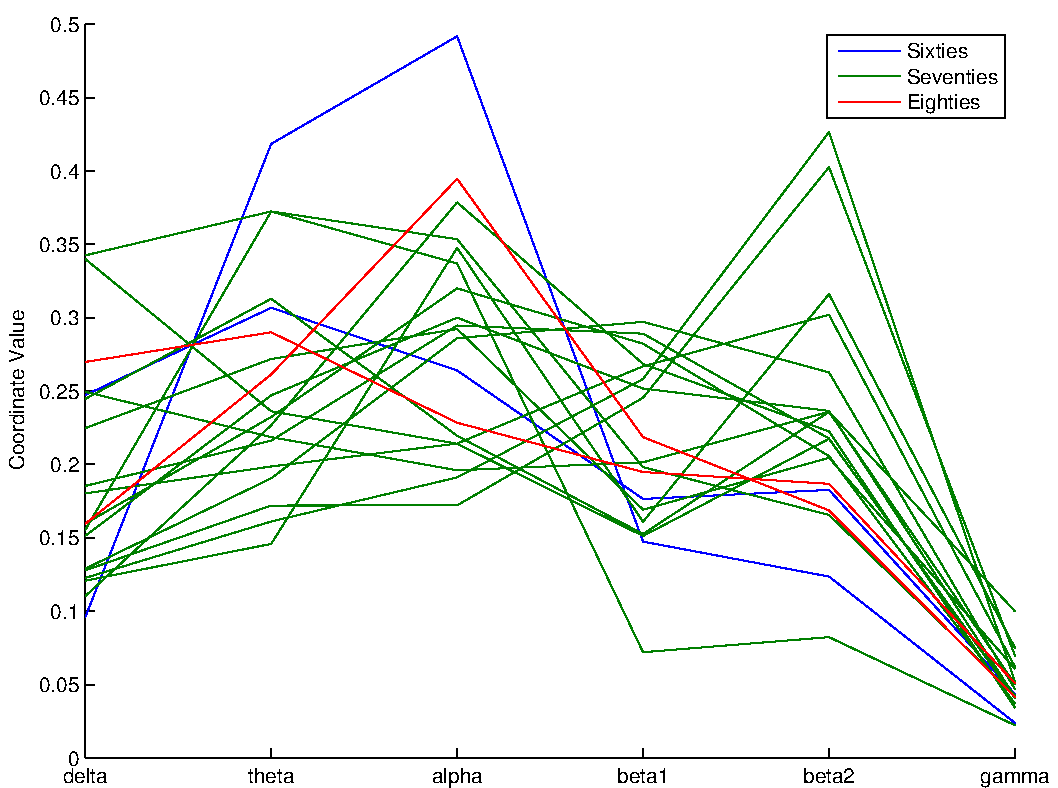
\includegraphics[width=.8\textwidth]{mciparacoords.pdf}
    \caption{The Parallel Coordinate Plot of the MCI dataset divided into different age groups, there is no discernable pattern or separation between them}
    \label{fig:mciparacoords}
\end{figure}


\begin{figure}[h]
  \centering
    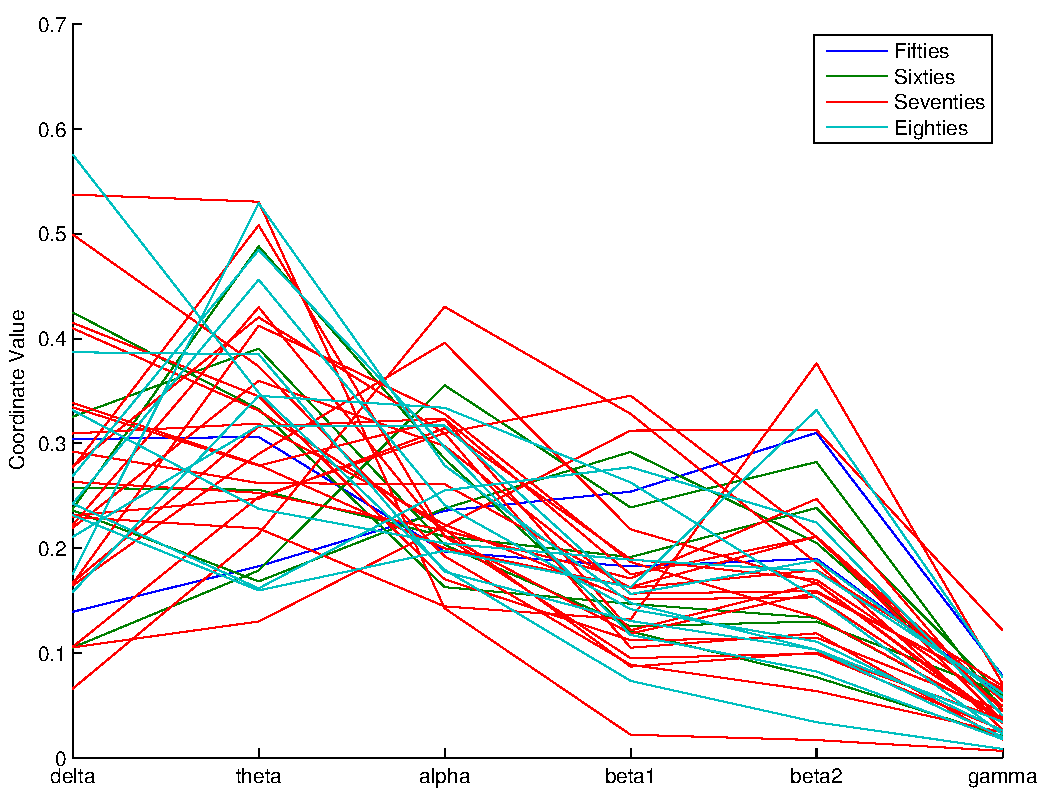
\includegraphics[width=.8\textwidth]{alzparacoords.pdf}
    \caption{The Parallel Coordinate Plot of the Alzheimer's dataset divided into different age groups, there is no discernable pattern or separation between them}
    \label{fig:alzparacoords}
\end{figure}

As can be seen in Figures \ref{fig:hparacoords}, \ref{fig:mciparacoords} and \ref{fig:alzparacoords} there was no clear distinction between the age groups which further explains why the model for predicting age from the relative powers wasn't very successful and corroborates the results of the t-SNE and PCA projections.

\clearpage
\subsection{Chernoff Faces}

A final and perhaps whimsical method of visualising multidimensional data is the \textit{glyph} based approach of Chernoff faces. These use the values of feature that a sample has to construct a human face, with the feature values being used to determine the size and shape of various parts of the face such as the eyes, mouth etc. The reasoning behind such a visualisation is that the human mind is adept at discerning the differences between human faces and thus can distinguish between relatively similar data more easily when it is presented in this manner. \cite{Chernoff1973}

The Chernoff Faces presented here used the reduced six feature set rather than the full set of 30 features because the Chernoff face package that was used did not have 30 tunable parameters. The features were used to determine the facial characteristics as follows in Table \ref{tab:chernoff}.


\begin{table}[h!]
\begin{center}
\begin{tabular}[h!]{|c|c|}
\hline
Relative Power Band & Chernoff Face Characteristic \\
\hline
Delta & Size of face \\
\hline
Theta & Forehead/jaw relative arc length \\
\hline
Alpha & Shape of forehead\\
\hline
Beta1 & Shape of jaw\\
\hline
Beta2 & Width between eyes\\
\hline
Gamma & Vertical position of eyes\\
\hline
\end{tabular}
\caption{The features and the corresponding facial characteristic in the Chernoff Face}
\label{tab:chernoff}
\end{center}
\end{table}

The datasets for the different classes were separated into the same age groups as before and averaged to produce `composite' Chernoff faces for each age group, note that the MCI dataset had no subjects aged 50-59 and thus it only has faces for the 60-69, 70-79 and 80-89 age groups.


\begin{figure}[h]
  \centering
    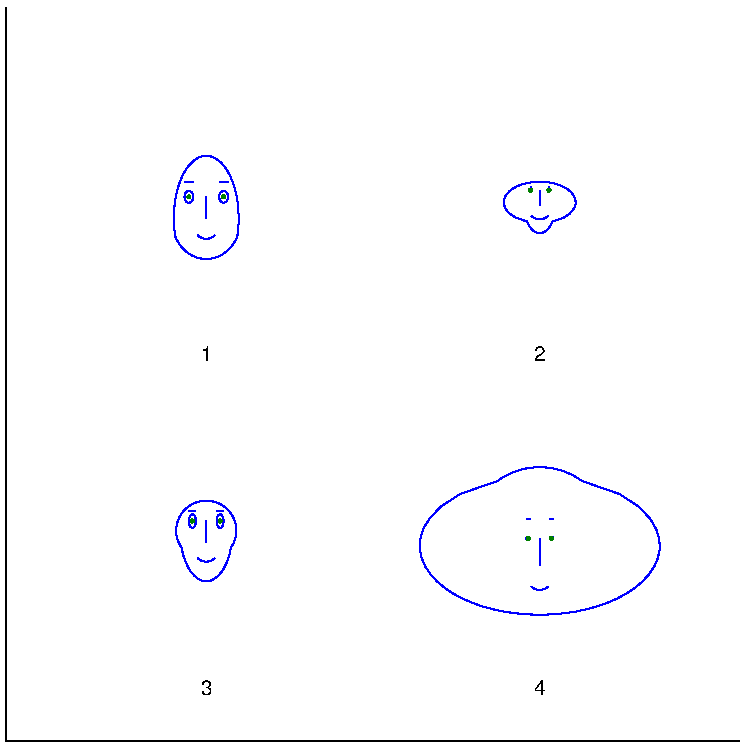
\includegraphics[width=.8\textwidth]{hChernoffFaces50607080.pdf}
    \caption{The Chernoff faces for the healthy dataset. Face 1 is age group 50-59, Face 2 is age group 60-69, Face 3 is age group 70-79, Face 4 is age group 80-89}
    \label{fig:hchernoff}
\end{figure}

\begin{figure}[h]
  \centering
    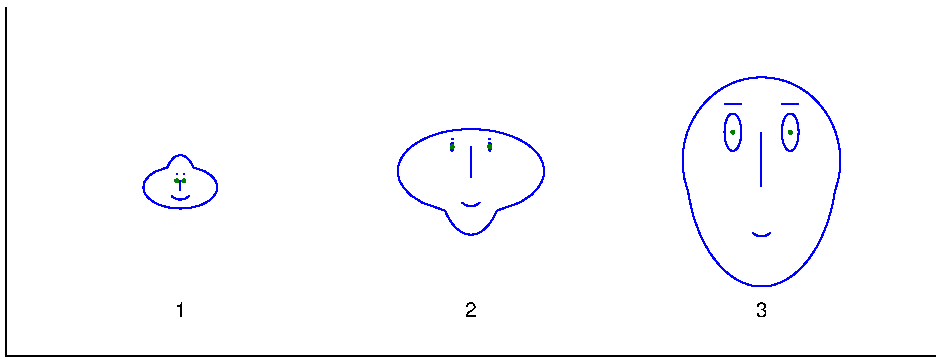
\includegraphics[width=.8\textwidth]{mciChernoffFaces607080.pdf}
    \caption{The Chernoff faces for the MCI dataset. Face 1 is age group 60-69, Face 2 is age group 70-79, Face 3 is age group 80-89}
    \label{fig:mcichernoff}
\end{figure}

\begin{figure}[h]
  \centering
    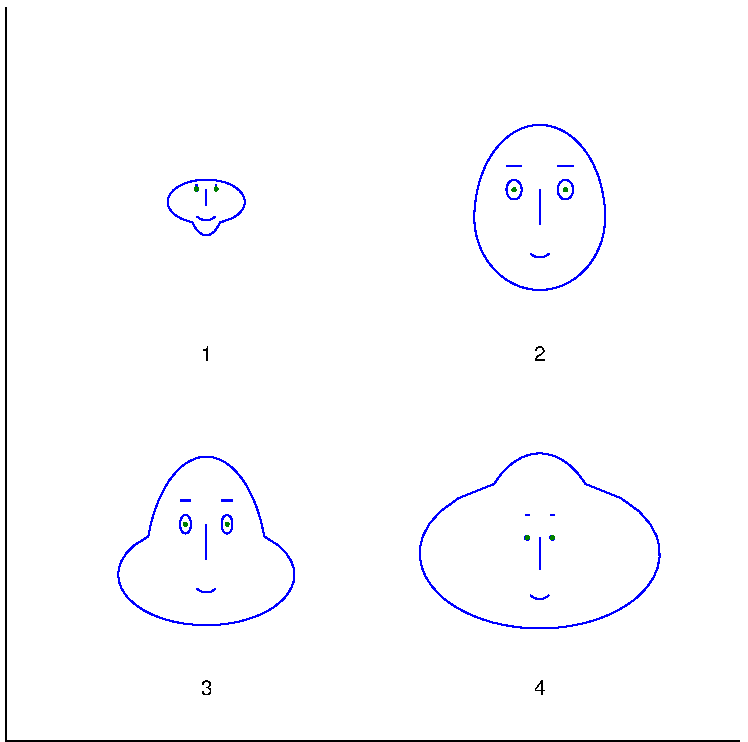
\includegraphics[width=.8\textwidth]{alzChernoffFaces50607080.pdf}
    \caption{The Chernoff faces for the Alzheimer's Disease dataset. Face 1 is age group 50-59, Face 2 is age group 60-69, Face 3 is age group 70-79, Face 4 is age group 80-89}
    \label{fig:alzchernoff}
\end{figure}

We can observe some differences between the age groups which perhaps explains why the age model didn't completely fail. However, as the relative differences between age groups seem the same in all the classes this implies that distinguishing between them will be very difficult, if possible, which supports the conclusions drawn from the previous visualisation techniques.



\clearpage


\section{Classification}

It was desired to classify a given subject as either healthy, suffering from MCI or suffering from Alzheimer's. This is an example of a \textit{supervised learning} problem as we have a fully labelled training and test set. As we have three classes it is \textit{multi-class classification} as opposed to the more common \textit{binary classification} problem when one has only two classes. Although any multi-class classification problem can be decomposed into several binary classification problem by training the same number of binary classifiers as classes with labels that are 1 for a certain class and 0 for all other classes. The test set is then classified according to which binary classifier most confidently predicted a value of 1. (One vs. All Classification) \cite{Witten2011}

RUSBoost was chosen as the classification algorithm because it is a ensemble multiclass classification algorithm that is robust to skewed classes in which the proportions of the classes present in the dataset is imbalanced.\cite{Seiffert2010} The data we have suffers from class imbalance as shown in Table \ref{tab:classimbalance} It is essentially an extension of the highly popular AdaBoost algorithm which uses adaptive boosting for classification and has been extended from binary to multiclass classification by the AdaBoost.M1 algorithm\cite{Witten2011}.

Adaptive boosting is an ensemble method which trains a series of weak learners and then uses a combination of their output (such as voting for classification) to classify the new sample. It is adaptive because each new weak classifier that is introduced is trained on a weighted training set and the weights are adjusted according to the success rate of previous classifiers on the samples. Therefore data samples which have not yet been classified correctly are given a high weight so that future classifiers will learn to classify them properly - this has the advantage that the combined strong classifier will know how to classify any data that is similar to that in the training set, but it also makes the algorithm highly sensitive to outliers.\cite{Witten2011}

To address class imbalance there are two possible strategies, one can either \textit{oversample} the minority classes  (e.g. sampling with replacement as in bootstrapping, creating synthetic data via interpolation of minority samples etc.) or one can \textit{undersample} the majority set (e.g. randomly leave out some of the majority class samples) until the desired class proportions are reached in the sample set.

RUSBoost utilises Random UnderSampling whereas an alternative SMOTEBoost uses Synthetic Minority Oversampling Technique (i.e. creating synthetic data by interpolation as mentioned previously). RUSBoost has been shown to have equal or better performance than SMOTEBoost with the additional advantages that as it uses a smaller training set it is quicker to train and as it doesn't require the generation of synthetic data is is much less computationally complex, this means that it is more efficient whilst still achieving an equal or better rate of classification accuracy. \cite{Seiffert2010}

\begin{table}[h!]
\begin{center}
\begin{tabular}[h!]{|c|c|c|}
\hline
Class & Count & Percentage of total data \\
\hline
Healthy & 220 & 79.14\% \\
\hline
AD & 39 & 14.03\% \\
\hline
MCI & 19 & 6.83\% \\
\hline
\end{tabular}
\caption{The proportion of classes in the data, note the imbalance}
\label{tab:classimbalance}
\end{center}
\end{table}




\begin{table}[h!]
\begin{center}
\begin{tabular}{cc|c|c|c|}
\cline{3-5}
& & \multicolumn{3}{c|}{Predicted Class} \\ \cline{3-5} & & Healthy & AD & MCI \\ \cline{1-5}
\multicolumn{1}{ |c| }{\multirow{2}{*}{Actual Class}} &\multicolumn{1}{ |c| }{Healthy} & 198 & 0 & 22\\ \cline{2-5}
\multicolumn{1}{ |c  }{}  & 
\multicolumn{1}{ |c| }{AD} & 22 & 6 & 11 \\ \cline{2-5}
\multicolumn{1}{ |c  }{}  & 
\multicolumn{1}{ |c| }{MCI} & 9 & 2 & 8 \\
\cline{1-5}

\end{tabular}
\caption{An example confusion matrix (from the model from the last fold of ten-fold cross-validation) for the classifier trained on the linear regression model residuals (all samples)}
\label{tab:residconfusion}
\end{center}
\end{table}





\begin{table}[h!]
\begin{center}
\begin{tabular}{cc|c|c|c|}
\cline{3-5}
& & \multicolumn{3}{c|}{Predicted Class} \\ \cline{3-5} & & Healthy & AD & MCI \\ \cline{1-5}
\multicolumn{1}{ |c| }{\multirow{2}{*}{Actual Class}} &\multicolumn{1}{ |c| }{Healthy} & 100 & 52 & 68\\ \cline{2-5}
\multicolumn{1}{ |c  }{}  & 
\multicolumn{1}{ |c| }{AD} & 7 & 24 & 8 \\ \cline{2-5}
\multicolumn{1}{ |c  }{}  & 
\multicolumn{1}{ |c| }{MCI} & 6 & 5 & 8 \\
\cline{1-5}

\end{tabular}
\caption{An example confusion matrix (from the model from the last fold of ten-fold cross-validation) for the classifier trained on the full feature set (30 features) of relative powers divided across the brain regions (all samples)}
\label{tab:fulldataconfusion}
\end{center}
\end{table}




The confusion matrices shown in Tables \ref{tab:residconfusion} and \ref{tab:fulldataconfusion} are taken from the final fold of cross-validation for classifiers fit to the residuals from the linear regression model and to the full feature set respectively. In the ideal case all of the examples would be on the leading diagonal of the matrix, as these are the correctly classified examples.

The average cross-validated classification accuracy across 10-fold was 76.26\% for the classifier trained on the residuals of the linear regression model and 47.48\% for the classifier trained on the complete relative power feature set. However a dummy classifier that simply predicted the majority class all the time would get a classification accuracy of 79.14\% despite being a useless classifier. Therefore it is better to use a figure of merit that takes into account the number of false positives and false negatives. One such measure for multi-class classification is the macro-averaged $F_1$ score. Which can be defined as the harmonic mean of the precision and recall values for each class, averaged over the classes.\cite{Sokolova2009} An $F_{1M}$ score of 1 is ideal, whilst 0 is the worst possible score. 

The general $F_{\beta M}$ score allows one to weigh the relative importance of precision and recall, i.e. the effects of false positive versus false negatives. In the multi-class case it is defined as:

\begin{equation}
F_{\beta M} = \frac{(\beta^2 +1) \textrm{Prec}_M \textrm{Rec}_M}{\beta^2 \textrm{Prec}_M + \textrm{Rec}_M}
\label{eq:fbeta}
\end{equation}

where the macro-averaged precision and recall values, $\textrm{Prec}_M$ and $\textrm{Rec}_M$ are defined as:

\begin{equation}
\textrm{Prec}_M = \frac{\sum\limits^{L}_{i=1} \frac{tp_i}{tp_i +fp_i}}{L}
\end{equation}

and
\begin{equation}
\textrm{Rec}_M = \frac{\sum\limits^{L}_{i=1} \frac{tp_i}{tp_i +fn_i}}{L}
\end{equation}

where $L$ is the total number of classes and $tp_i$, $fp_i$ and $fn_i$ are the number of true positives, false positives and false negatives for that class respectively. Note that the $F_{1M}$ is simply calculated using Equation \ref{eq:fbeta} with $\beta = 1$


The $F_{1M}$ scores were 0.542, 0.458 and 0.294 for training on the linear regression model residuals, the full feature set and from the dummy classifier respectively. 

The classifiers consisted of a boosted ensemble of 1500 decision trees. As shown in Figures \ref{fig:resid1500treesCVerror} and \ref{fig:full1500treesCVerror} the classification error began to plateau at 1500 weak learners and adding more and more would eventually lead to overfitting and an increasing error rate, but as it was computationally expensive and even 1500 learners was quite time-consuming to train ($\approx30$ minutes training time) it seemed appropriate to stop once such diminishing returns were observed.



\begin{figure}[h!]
  \centering
    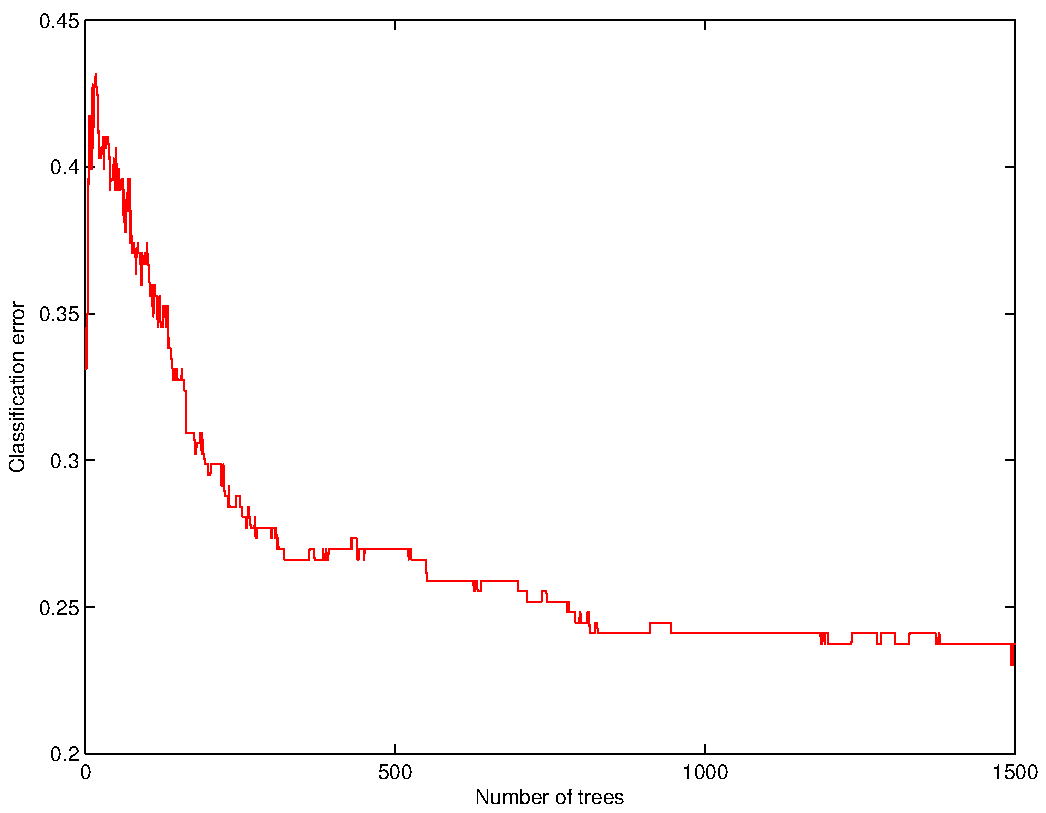
\includegraphics[width=.8\textwidth]{resid1500treesCVerror.pdf}
    \caption{The classification error plotted as a a function of the number of weak classifiers for the ensemble trained on the residuals of the linear regression model}
    \label{fig:resid1500treesCVerror}
\end{figure}



\begin{figure}[h!]
  \centering
    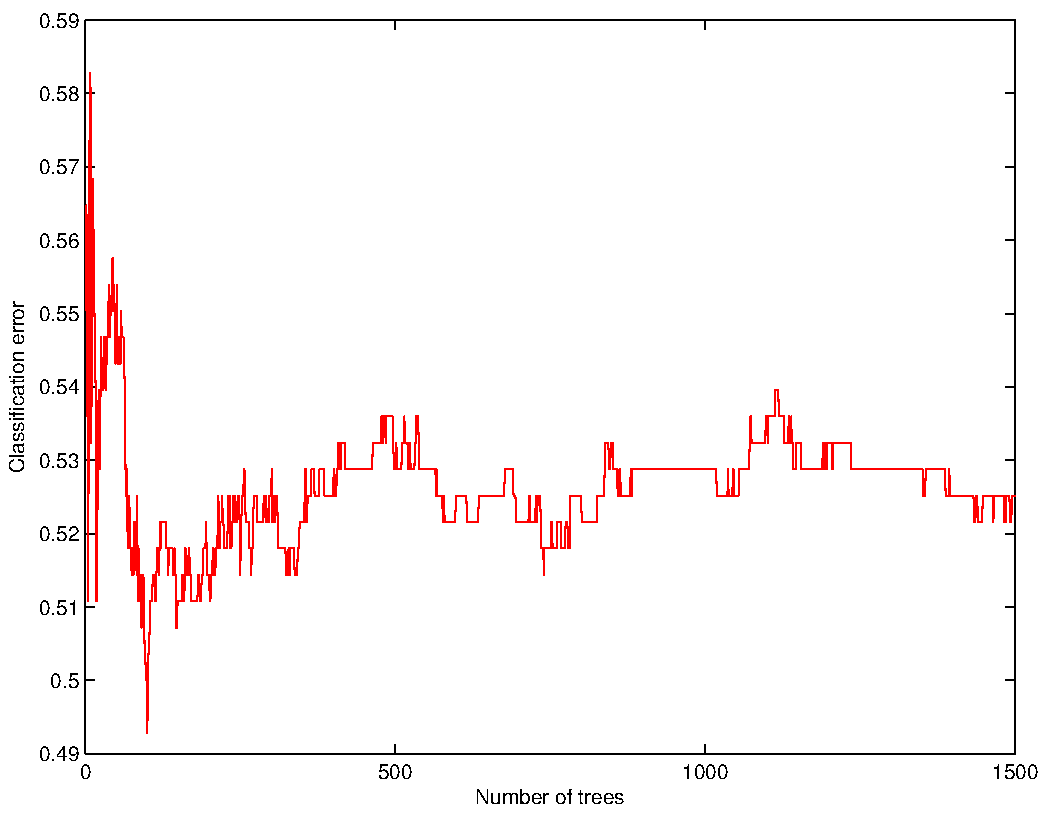
\includegraphics[width=.8\textwidth]{full1500treesCVerror.pdf}
    \caption{The classification error plotted as a a function of the number of weak classifiers for the ensemble trained on the full feature set of thirty relative powers}
    \label{fig:full1500treesCVerror}
\end{figure}




  \chapter{Analysis and Evaluation}

Despite the early positive results from the RMSE values of the linear regression model once the classes did not appear to be separable in the visualisations produced it seemed unlikely that the classification attempt would be highly successful. Although previous work \cite{Gomez2013} had related the relative powers to the age of the subject via a quadratic relationship, an attempt to fit a quadratic model to the data we had was less successful than the linear model. It is worth noting that the previous study investigated the relative powers as a function of age, looking at each relative power band separately and thus it simple linear regression rather than multiple regression, and our study investigated the age as a function of the relative powers. The difference are because of the different aims of the studies, they were investigating the effect of age on the relative powers, whereas we were attempting to predict the age from the relative powers.

Although the RMSE values obtained from the linear model do agree with our expectations (the healthy data has significantly less error than the MCI data which has less error than the AD data), they are still quite large especially the value of 14.86 years for the healthy dataset, which given that the model is trained on the healthy data should be very low as the model should be able to predict it very well. Of course given that the diseased patients had significantly worse RMSE values that should not prevent the residual values from being used to classify the disease, but it does show that the data is perhaps quite noisy or the relative powers just have little information about the age of the subject.

The correlation observed between the residuals of the model and the cognitive test scores for the diseased patients was very weak as demonstrated by the poor $r^2$ values, therefore it appears that the difference in relative powers between diseased and healthy patients (which the model residual effectively acts as a proxy for) is not sufficient to determine the severity of the disease. Also it should be noted that the predicted age for the diseased patients was often lower than their actual age. This doesn't fit the hypothesis that the difference in the model would reflect accelerated brain ageing.

It is interesting to see that the classifier trained solely on the residuals from the model did better than that using the whole feature set. This is probably due to the \textit{curse of dimensionality} in which the high-dimensional space of the larger feature set causes the classifier to perform poorly \cite{Witten2011}. The residuals of the linear regression models are based on the relative powers and so in principle should contain much the same information (i.e. it is essentially a form of feature engineering), but the dimensionality has been reduced, thus allowing the classifier to perform better. It should also be noted that boosted algorithms perform very poorly in the case of label noise (mislabelled training examples) \cite{Long2009}. This is important to note in our case as Alzheimer's and MCI diagnosis is not an exact science and some of the subjects may have been misdiagnosed.

A `dumb' classifier that simply predicted all the patients to be healthy would outperform it (based purely on classification accuracy). The fact that the classifier didn't just learn to classify all patients as healthy shows that RUSBoost is successful at dealing with skewed classes but nonetheless the classifier is still not successful enough to be useful, especially in medical diagnosis which requires a classifier to be both highly sensitive and highly specific (i.e. a low false positive and false negative rate) because of the economic costs of unnecessary tests and treatments alongside the psychological strain of a false diagnosis whilst a false negative result can have potentially fatal consequences.

The $F_{1M}$ score that takes false positives and false negatives into account and is thus often a better figure of merit than classification accuracy (especially for medical diagnosis where the mistakes are important as previously discussed) favoured our classifiers over the dummy classifier but as mentioned previously they are far from the quality required for medical diagnosis.

There were some difficulties with the study, for example because MCI and Alzheimer's are typically diagnosed in old age this means that some of the inaccuracy of the model may simply be due to the fact that it was also trained on younger healthy ages, whereas the AD and MCI patients were all relatively old. This is compounded by the fact that most of the control subjects were younger perhaps because students are common participants in such experiments and they tend to be young.

Furthermore given the nature of resting-state MEG experiments it is somewhat common for the subjects to fall asleep as it is dark, the subject is asked to remain immobile and the experiment may last quite some time. This is not a problem in itself if it is correctly reported, but even with a camera it can be very difficult to notice if the subject has fallen asleep and while healthy subjects are usually aware that they have fallen asleep upon waking, diseased patients who are cognitively impaired may fail to report it thus leading to contaminated data. This often shows up in the power spectra as an increased power in the lower frequency bands, but manually inspecting every power spectrum is not feasible given the vast number of subjects, channels and epochs. Given that the instances in which the subject falls asleep are rare compared to the awake state it is possible that in the future one could attempt to use anomaly detection methods\cite{Chandola2009} to detect the contaminated epochs.

The healthy dataset was composed of a combination of control groups from various experiments in order to get a sufficient sample size, however this could cause problems if the data was affected by the fact it was recorded over a long time period (months and years, rather than days). However, given the relative powers were used rather than absolute measures and the artefact rejection was conducted on a `per subject' basis this seems unlikely.




  \chapter{Conclusion and future works}



  % Appendix
  %\appendix

  %\chapter{Tools}




  % Bibliography
  \bibliography{refs/bibliography}{}
  \bibliographystyle{apalike}
\end{document}
